\documentclass[12pt]{article}

%--------------------------------------------------------
% Basic Page Setup
%--------------------------------------------------------
\usepackage[margin=1in]{geometry} 
\usepackage{lmodern}
\usepackage[T1]{fontenc}
\usepackage[utf8]{inputenc}
\usepackage{microtype}  % Improves typography
\usepackage{pgfplots}
\pgfplotsset{compat=newest}  % Use the latest available features


% Slightly increase line spacing
\renewcommand{\baselinestretch}{1.2}

%--------------------------------------------------------
% Math Packages
%--------------------------------------------------------
\usepackage{amsmath,amssymb,amsthm}

%--------------------------------------------------------
% tcolorbox for Call-Out Blocks
%--------------------------------------------------------
\usepackage{tcolorbox}
\usepackage{xcolor}
\tcbuselibrary{theorems}

\definecolor{custom_green}{HTML}{a3be8c}
\definecolor{custom_red}{HTML}{bf616a}
\definecolor{custom_blue}{HTML}{5e81ac}
% Definition box
\newtcolorbox{definitionbox}{
  title=Definition,
  fonttitle=\bfseries,
  colback=blue!5!white,    % Light blue background
  colframe=blue!30!white,  % Darker blue frame
  coltitle=black,
  boxrule=1.5pt,
  arc=3pt,
  outer arc=3pt,
}

% Theorem box
\newtcolorbox{theorembox}{
  title=Theorem,
  fonttitle=\bfseries,
  colback=custom_green!30!white,
  colframe=custom_green,
  coltitle=black,
  boxrule=0.5pt,
  arc=4pt,
  outer arc=4pt,
}

% Note box
\newtcolorbox{examplebox}{
  title=Example,
  fonttitle=\bfseries,
  colback=custom_red!20!white,
  colframe=custom_red,
  coltitle=white,
  boxrule=0.5pt,
  arc=4pt,
  outer arc=4pt,
}


\newtcolorbox{proofbox}{
  title=Proof,
  fonttitle=\bfseries,
  colback=custom_blue!20!white,
  colframe=custom_blue,
  coltitle=white,
  boxrule=0.5pt,
  arc=4pt,
  outer arc=4pt,
}

\newtcolorbox{corollarybox}{
  title=Corollary,
  fonttitle=\bfseries,
  colback=custom_blue!20!white,
  colframe=custom_blue,
  coltitle=white,
  boxrule=0.5pt,
  arc=4pt,
  outer arc=4pt,
}

%--------------------------------------------------------
% Theorem Environments (optional alternative)
%--------------------------------------------------------
\theoremstyle{definition}
\newtheorem{definition}{Definition}[section]
\newtheorem{example}[definition]{Example}

\theoremstyle{plain}
\newtheorem{theorem}[definition]{Theorem}


\title{
Complex Analysis\\[2ex]
Exams:\\
60\% Exam\\
40\% Continuous Assessment
}
\author{}     % Optional: Add author details if desired
\date{}       % Optional: Add date if desired
%--------------------------------------------------------
% Document
%--------------------------------------------------------
\begin{document}
\maketitle
\pagebreak

\tableofcontents
\pagebreak

\section{Week 1: Introduction to Complex Numbers}
\subsection{Quadratics with Complex Roots}
Everybody knows that, for coefficients $a,b,c \in \mathbb{R}$, the quadatric
$$ax^2 + bx +c = 0$$
has real values solutions given by:
$$x = \dfrac{-b\;\pm\;\sqrt{b^2 - 4ac}}{2a}\quad\quad\quad \text{if } b^2 -4ac \geq 0$$ 
but if $b^2 - 4ac < 0$, then we need the roots of negative numbers, and thus the solutions are complex numbers.\\
For example, the, the plot of $x^2 + 1 = 0$, below implies imaginary soltuons, since there are no real $x$-values that make y=0
\begin{center}
  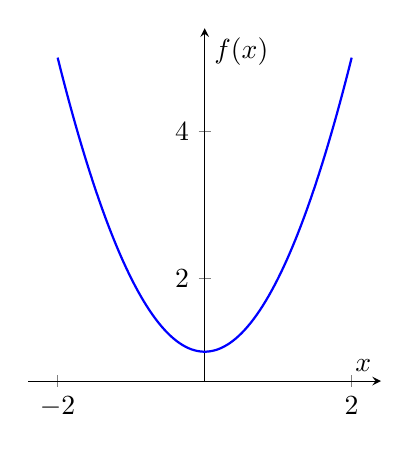
\begin{tikzpicture}
    \begin{axis}[
        width = 0.5\textwidth,
        height = 0.5\textwidth,
        axis lines = middle,
        xlabel = {$x$},
        ylabel = {$f(x)$},
        domain = -2:2,
        samples = 100,
        enlargelimits = true
      ]
      \addplot [blue, thick] {x^2 + 1};
    \end{axis}
  \end{tikzpicture}
\end{center}
\newpage
\subsection{Real valued solutions of a cubic}
Oddly enough, complex numbers are needed to find real-valued solutions of a cubic equation.
\begin{definitionbox}
  For $p, q \in \mathbb{R}$, 
$$x^3 = px + q,$$
has the solution, by Cardano's formula:
  $$x = \sqrt[3]{\frac{q}{2} + \sqrt{\left(\frac{q}{2}\right)^2 - \left(\frac{p}{3}\right)^3}} + \sqrt[3]{\frac{q}{2} - \sqrt{\left(\frac{q}{2}\right)^2 - \left(\frac{p}{3}\right)^3}}$$
\end{definitionbox}

\begin{examplebox}
Consider $x^3 = 15x +4$, staring at this long enough, one could guess that $x=4$ is a solution, and then factor out $(x-4)$ to get a quadratic, but that's not the point.\\
By Cardano's Formula, with $p = 15$ and $q = 4$, we get:
$$\sqrt[3]{2 + \sqrt{-121}} + \sqrt[3]{2-\sqrt{121}}$$
Setting $i = \sqrt{-1}$, thus $\sqrt{-121} = 11i$ \\
And noticing that:
\begin{align*}
  (2+i)^3 &= 2^3 + 3\cdot2^2 \cdot i + 3\cdot 2 \cdot i^2 + i^3 \\
  &= 8 + 12i - 6 - i \\ 
  &= 2 + 11i \\ 
  \text{Thus} \quad (2+1)^3 = 2 + 11i \quad &\text{and} \quad (2-1)^3 = 2 - 11i
\end{align*}

Thus, the solution is:
\begin{align*}
  &= \sqrt[3]{(2+i)^3} + \sqrt[3]{(2-i)^3} \\ 
  &= 2+ i + 2 - i \\
  &= 4
\end{align*}
\end{examplebox}
\pagebreak
\subsection{Definition of Complex Numbers}

\begin{definitionbox}
  The set of complex numbers is defined as: 
  $$\mathbb{C} = \{x + yi \mid x,y \in \mathbb{R}\}$$
  where $a$ is the real part and $yi$ is the imaginary part, and $i^2 = -1$
\end{definitionbox}
\subsection{Attributes of Complex Numbers}
Given a complex number of the form: $z = x + yi$, we have:
\begin{itemize}
  \item Re$(z) = x$ is the real part of $z$ \
  \item Im$(z) = y$ is the imaginary part of $z$ 
  \item $\bar{z} = x - yi$ is the complex conjugate of $z$
  \item $|z| = \sqrt{x^2 + y^2}$ is the modulus of $z$
\end{itemize}
Note that: 
\[
z\bar{z} = x^2 + y^2 = |z|^2 \in \mathbb{R}
\]
Also note how this formula is used in the computation of the inverse of $z$:
\[
z^{-1} = \frac{\overline{z}}{|z|^2}
\]
The geometric meaning of these attributes can be seen below.
  \begin{center}

  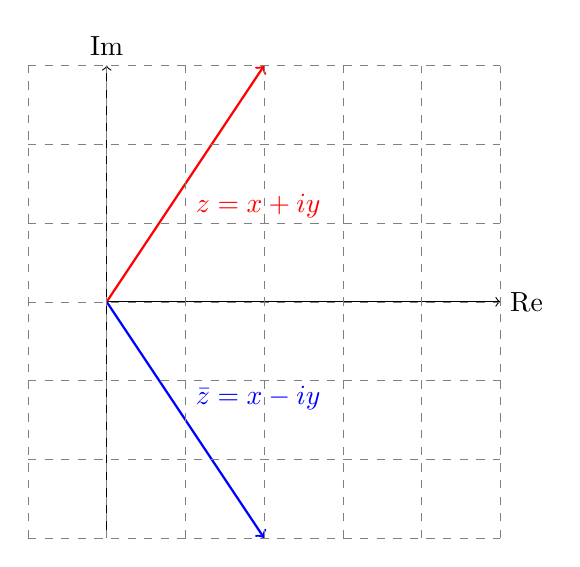
\begin{tikzpicture}
    % Draw the axes
    \draw[->] (0,0) -- (5,0) node[right] {$\mathrm{Re}$};
    \draw[->] (0,-3) -- (0,3) node[above] {$\mathrm{Im}$};
  
    % Draw the vectors
    \draw[->,thick,red] (0,0) -- (2,3) node[midway, below right] {$z = x + iy$};
    \draw[->,thick,blue] (0,0) -- (2,-3) node[midway, above right] {$\bar{z} = x - iy$};
  
    %Add grid lines
    \draw[help lines, dashed, gray] (-1,-3) grid (5,3);
  \end{tikzpicture}
\end{center}

\pagebreak 

\subsection{Polar Form of a Complex Number}
Given a non zero complex number $z = x + iy$:
\begin{enumerate}
  \item \textbf{Magnitude}: $\mid z \mid = \sqrt{x^2 + y^2}$
  \item \textbf{Argument}: If you think of $(x,y)$ as a point in the plane, $\theta$, is the angle the vector from the origin makes with the positive $x-axis$
  \begin{itemize}
    \item In polar form, we write: $z = |z|(\cos\theta + i\sin\theta)$
    \item \textbf{Principle Argument} (Arg z): This is the "main" angle $\theta$ chosen to lie in $(-\pi, \pi]$
    \item Because angles can differ by full turns $(2\pi)$, the general argument of $z$ can be written as: $$\text{arg}(z) = \text{Arg}(z) = 2\pi n, \quad n \in \mathbb{Z}$$
  \end{itemize}
\end{enumerate}

\noindent \textbf{Why angles are "multi-valued"}
A direction in the plane can be expressed by infintetly many angles differing by whole circle $(2\pi)$. The "principal" angle is just a standard choice in $(-\pi, \pi]$

\subsection{Multplication by $i$ and Geometric Interpretation}
Multiplying a complex number $z$ by $i$ correspond to a rotation by $\frac{\pi}{2}$ (90$^\circ$) in the complex plane.. \\ 
Example:
\begin{align*}
  z &= x + iy \\
  iz &= i(x + iy) \\
  &= ix - y \\
  &= -y + ix
\end{align*}

\begin{center}
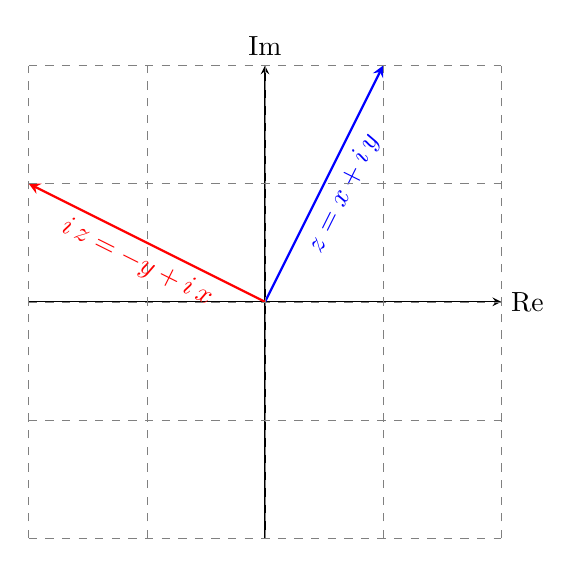
\begin{tikzpicture}[>=stealth, scale=1.5]
  % Axes
  \draw[->] (-2,0) -- (2,0) node[right] {$\mathrm{Re}$};
  \draw[->] (0,-2) -- (0,2) node[above] {$\mathrm{Im}$};

  % Define x and y (feel free to change these)
  \def\x{1}
  \def\y{2}

  % Plot z = x + i y
  \draw[thick,->,blue] (0,0) -- (\x,\y)
      node[midway,sloped, below] {$z = x + i\,y$};

  % Plot i z = -y + i x
  \draw[thick,->,red] (0,0) -- (-\y,\x)
      node[midway,sloped,below] {$i\,z = -y + i\,x$};

  % Optional: add a grid
  \draw[help lines,dashed] (-2,-2) grid (2,2);
\end{tikzpicture}
\end{center}

\subsection{Products of Complex Numbers and De Moivre's Theorem}
\begin{theorembox}
Let $z, z' \in \mathbb{C} \backslash \{0\}$, then:
\begin{itemize}
  \item $|zz'| = |z||z'|$ and $\left|\dfrac{z}{z'}\right| = \dfrac{|z|}{|z'|}$
  \item Arg$(zz')$ = arg$(z)$ + arg$(z')$ and arg$\left(\dfrac{z}{z'}\right)$ = arg$(z)$ - arg$(z')$
\end{itemize}
\end{theorembox}

\begin{proofbox}
Let $x - x + iy$ and $x' + iy'$, thus:
$$z = |z|(\cos\theta + i\sin\theta) \quad \text{and} \quad z' = |z'|(\cos\theta' + i\sin\theta')$$
Then:
\begin{align*}
|zz'| &= |z||z'|(\cos\theta + i\sin\theta)(\cos\theta' + i\sin\theta') \\
&= |z||z'|\left[(\cos\theta\cos\theta' - \sin\theta\sin\theta' + i(\cos\theta\sin\theta' + \sin\theta\cos\theta'))\right] \\
&= |z||z'|\left[\cos(\theta + \theta') + i\sin(\theta + \theta')\right] \\
\end{align*}

Thus, $|zz'| = |z||z'|$ and arg$(zz') = \theta + \theta' = \text{arg}(z) + \text{arg}(z')$ \\
Note that: $|z||z'|$ acts as a stretch/ shrink, $\cos(\theta + \theta')$ and $\sin(\theta + \theta')$ act as a rotation. 
\end{proofbox}

\begin{corollarybox}
\textbf{De Moivre's Thereom:} If $z = |z|(\cos\theta + i\sin\theta)$, then:
$$z^n = |z|^n \cos(n\theta) + i sin(\theta)$$
\end{corollarybox}

\noindent De Moivre's Thereom is extemely useful for raising a complex number to inger powers and expressing $nt$th roots of unity (as a special case where $r=1$ and $z^n = 1$)

\pagebreak

\subsection{Roots of Unity}
A \textbf{root of unity} is a complex number $z$, such that:
$$z^n = 1 \quad \text{for some integer} n \geq 1$$
Geometrically, roots of unity lie on the unit circle in the complex plane.\\
Specifically:
\begin{definitionbox}
  The $n$th roots of unity are given by:
  $$z_k = \cos\left(\frac{2\pi k}{n}\right) + i\sin\left(\frac{2\pi k}{n}\right) \quad \text{for } k = 0,1,2,\ldots,n-1$$
\end{definitionbox}


\begin{examplebox}
    Recalling $z = |z|\left[\cos\theta + i\sin\theta\right]$ \\
    Letting $z^4 = 1$, then we see:
    \begin{align*}
      z^4 &= \cos(4\theta) + i\sin(4\theta) =1 + 0i\ 
    \end{align*}

    We see, $z$ is one of $w_k = \cos\left(\frac{2\pi k}{4}\right) + i\sin\left(\frac{2\pi k}{4}\right) = 1, i,-1, i$\\
    And that the 4 roots of unity form a square in the unit circle, and their sum is 0.
\end{examplebox}


\section{Week 2: Functions of a Complex Variable}

\end{document}
